\documentclass{article} % For LaTeX2e
\usepackage{nips14submit_e,times}
\usepackage{hyperref}
\usepackage{url}
\usepackage{amsmath}
\usepackage{amssymb}
\usepackage{algorithm}
\usepackage[noend]{algpseudocode}
\usepackage{graphicx}
\usepackage[labelfont=bf]{caption}
%\documentstyle[nips14submit_09,times,art10]{article} % For LaTeX 2.09

\DeclareMathOperator{\rvec}{rvec}

\title{RNN-RNADE: A Tractable Model for High-Dimensional Real Valued Sequences}


\author{
David S.~Hippocampus\thanks{ Use footnote for providing further information
about author (webpage, alternative address)---\emph{not} for acknowledging
funding agencies.} \\
Department of Computer Science\\
Cranberry-Lemon University\\
Pittsburgh, PA 15213 \\
\texttt{hippo@cs.cranberry-lemon.edu} \\
\And
Coauthor \\
Affiliation \\
Address \\
\texttt{email} \\
\AND
Coauthor \\
Affiliation \\
Address \\
\texttt{email} \\
\And
Coauthor \\
Affiliation \\
Address \\
\texttt{email} \\
\And
Coauthor \\
Affiliation \\
Address \\
\texttt{email} \\
(if needed)\\
}

% The \author macro works with any number of authors. There are two commands
% used to separate the names and addresses of multiple authors: \And and \AND.
%
% Using \And between authors leaves it to \LaTeX{} to determine where to break
% the lines. Using \AND forces a linebreak at that point. So, if \LaTeX{}
% puts 3 of 4 authors names on the first line, and the last on the second
% line, try using \AND instead of \And before the third author name.

\newcommand{\fix}{\marginpar{FIX}}
\newcommand{\new}{\marginpar{NEW}}

%\nipsfinalcopy % Uncomment for camera-ready version

\begin{document}


\maketitle

\begin{abstract}
We present a probabilistic model for generating and modelling high dimensional real-valued sequences. This model combines a powerful distribution estimator, the Real-Valued Neural Autoregressive Density Estimator (RNADE) with a Recurrent Neural Network (RNN) for capturing temporal dependencies in sequences of high dimensional data. Maximum likelihood learning can be applied to efficiently train the model using a gradient based optimiser. Unlike other models in this family, log-likelihoods for sequences can be computed exactly and efficiently. We evaluate the model's performance on standard datasets and report a significant 55\% relative improvement on the \textit{mocap} dataset. 
\end{abstract}

\section{Introduction}
\label{intro}
Modeling sequences is a fundamental problem in machine learning. Speech, music, video and many kinds of naturally occurring data are sequential in nature. A good sequential model can be used for discriminative tasks, for sequence completion, as a prior in more complex tasks, for sequence denoising and for various other applications. There are several existing approaches such as Linear Dynamical Systems and Hidden Markov Models (HMMs) that can model sequential data. Although these systems are used extensively in many fields such as speech, audio and music, they can only model a limited history, meaning that capturing long term dependencies between data points becomes intractable \cite{sutskever2007learning}. 

Recurrent Neural Networks (RNNs) are powerful systems for modelling sequential data. RNNs have an internal memory that allows them to capture dependencies between observations separated by a variable number of time steps. In principle RNNs can describe relationships between inputs separated by arbitrary lengths of time. However, in practice, training RNNs using gradient based optimisers is not easy and their use in practical applications has been limited \cite{bengio2012advances}. After being ignored by machine learning researchers for a long time, there has been a resurgence of interest in RNNs. Over the last decade, there have been several key developments in understanding and solving some of the issues associated with gradient based training of RNNs \cite{Martens2011,bengio2012advances}. These advances have made it possible to train RNNs on a variety of tasks and they have been shown to be very successful on a large number of music and language applications \cite{mikolov2011empirical,Boulanger-Lewandowski2012,bengio2012advances}. 

An RNN can either be used to map an input sequence to an output sequence or it can be used as a generative model. Generative models attempt to model the entire space of inputs given a finite number of training examples. In a standard RNN architecture, when predicting multivariate outputs, the outputs at time $t$ are conditionally independent given the sequence up until time $t$. However, for many problems this assumption of conditional independence does not hold. Dependencies between the output variables can be modelled by using the RNN to predict the parameters of a powerful distribution estimator, similar to the architecture of a mixture density network \cite{bishop1994mixture}. Employing this architecture complex high-dimensional distributions can be produced at each time-step, conditioned on the previous inputs. This idea was first employed in the Recurrent Temporal Restricted Boltzmann Machine (RTRBM) \cite{Sutskever2008}. The system was then extended by combining an RNN with a Neural Autoregressive Distribution Estimator (NADE) and an RBM via a more general architecture \cite{Boulanger-Lewandowski2012}. The RNN-RBM and RNN-NADE have been successfully applied to tasks in speech and music \cite{boulangerphone,Boulanger-Lewandowski2012}. 

Although the models described above have been successful on many tasks, they are unsuitable for modelling real-valued data. Both the RBM and the NADE are designed to explicitly model binary vectors. If the input data lies in $[0,1]$, then the RBM can be used with the mean-field approximation to produce real values. Unbounded data can be modelled by using Gaussian visible units and Bernoulli hidden units. However, these extensions of the RBM to real data have several known limitations \cite{theis2011all}. In this paper, we present a new model for real-valued sequential data by combining the RNN with the RNADE. The RNADE is a density estimator that has been shown to outperform Gaussian mixture models (GMMs) and a host of other density estimators on several tasks \cite{Uria2013}. We show that obtaining probabilities and log-likelihoods from the combined RNN-RNADE model is tractable and fast. We show that the gradients with respect to the model parameters can be calculated exactly and that training can be easily performed with a gradient based optimiser. We evaluate the model's performance on real-valued datasets and demonstrate a marked improvement in performance on the {\it \textit{mocap}} dataset, which is described in Section \ref{Experiments}. 
 
\section{Recurrent Neural Networks as generative models}
\label{RNN}
\begin{figure}
        \centering
    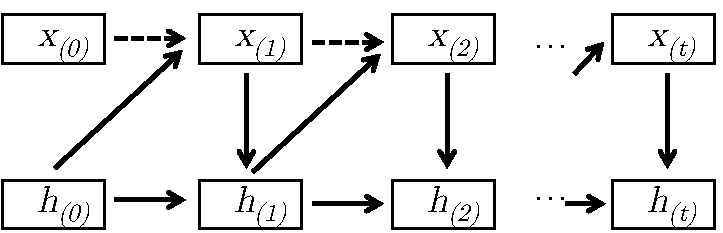
\includegraphics[scale=0.8]{RNN.pdf}
    \caption{Graphical structure of the generative RNN. Broken arrows indicate optional connections for temporal smoothing.}
    \label{fig:rnn}
\end{figure}


An RNN defines a distribution over an output sequence $ \mathbf{x} \equiv \left\{ \mathbf{x}^t \in \mathbb{R}^n, t \leq T \right\}$ in the following manner:
$$ P(\mathbf{x}) = \prod_{t=1}^{T} P(\mathbf{x}^t|\mathcal{A}^t)$$
where $\mathcal{A}^t \equiv \left\{ \mathbf{x}^{\tau}|\tau < t \right\}$ is the history of the input sequence $\mathbf{x}$ until time $t$, $P(\mathbf{x}^t|\mathcal{A}^t)$ is the probability of observing $\mathbf{x}^t$ conditioned on the history of the sequence $\mathcal{A}^t$ and $T$ is the number of time-steps in the sequence. RNN based generative models with different properties and capacities can be constructed by carefully choosing the form and parameterisation of the conditional $P(\mathbf{x}^t|\mathcal{A}^t)$ as discussed later in this section. 

In an RNN with a single hidden layer, the hidden state at time $t$ is given by:
\begin{equation}
\label{rnn-hidden}
\mathbf{h}^t = \sigma{(W_{in}\mathbf{x}^t + W_{rec}\mathbf{h}^{t-1} + \mathbf{b}_h)}
\end{equation}
where $W_{in}$ is the weight matrix from the input to the hidden layer, $W_{rec}$ is the recurrent weight matrix from the previous hidden state to the current state and $\mathbf{b}_h$ is the bias vector for the hidden layer. In a standard RNN, the next time step $\mathbf{x}^{t+1}$ is predicted as:
$$ \mathbf{x}^{t+1} = \sigma{(W_{out}\mathbf{h}^{t} + \mathbf{b}_{out})}$$  
where $W_{out}$ connects the hidden layer to the output layer and $\mathbf{b}_{out}$ is the output bias. As shown in Figure \ref{fig:rnn}, there can be optional connections between the input and the input from the previous time-step for temporal smoothing. However, as mentioned earlier, each of the outputs is conditionally independent given the input sequence. This assumption is too restrictive for many real-world problems and has lead to a new family of RNN-based generative models with high-dimensional multi-modal conditional distributions at each time-step. Such a model can be realised by letting the hidden layer of the RNN predict parameters of a distribution estimator. 

In previous work \cite{Boulanger-Lewandowski2012}, the RNN was used to predict the hidden and visible biases of an RBM and a NADE model to yield complex conditional distributions at each time step. Although these models are very good at modelling sequences of binary vectors, they are unsuitable for modelling real-valued data. It is easy to show that any distribution estimator can be used provided the gradients of the cost function with respect to the parameters of the density estimator are obtainable. The combined model can then be trained by maximising the likelihood of the training set and using back-propagation through time (BPTT) \cite{rumelhart1985learning}. In order to use the power of this architecture for modelling real data, we present a model that combines the RNN and the RNADE. The RNADE is discussed in detail in the following section and the combined model is described in Section \ref{RNN-RNADE}. 

\section{The RNADE}
\label{RNADE}
\begin{figure}
        \centering
    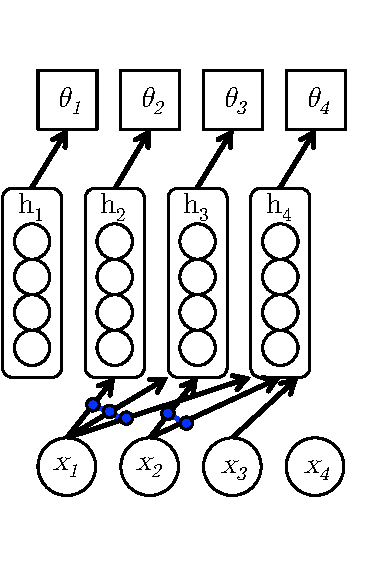
\includegraphics[scale=0.7]{RNADE.pdf}
    \caption{
Graphical structure of the RNADE. The blue dots indicate that the weights coming out from a node are tied. $\theta_{d}$ denote the parameters of the mixture density network for the dimension $d$. }
    \label{fig:rnn-rnade}
\end{figure}


The RNADE is a generalisation of the NADE to model real-valued data. Like the NADE, the RNADE expresses the joint probability of the data as a product of one-dimensional conditional distributions as follows:
$$ p(x) = \prod_{d=1}^{D} p(x_d|\mathbf{x_{<d}}) \: \text{with} \: p(x_d|\mathbf{x_{<d}}) = p_{\mathcal{M}(x_d|\theta_d)} $$ where $p_{\mathcal{M}}$ is a mixture of Gaussians, $\boldsymbol{x}_{<d}$ is a vector of the first $d-1$ dimensions of $x$ and $D$ is dimensionality of the input space. The RNADE is computationally efficient because of the weight sharing employed in the calculation of the hidden state: 

$$ \mathbf{a}_d = \boldsymbol{W}_{.,<d}\boldsymbol{x}_d + \mathbf{c}$$
$$ \boldsymbol{h}_d = \sigma (\rho_d \mathbf{a}_d)$$


where $\mathbf{c} \in \mathbb{R}^{H}$ and $\boldsymbol{W} \in \mathbb{R}^{D \times (H-1)}$ are parameters that are shared across all the feed forward neural networks and $\sigma(x) = 1/(1+e^{-x})$ is the sigmoid function. $\boldsymbol{W}_{.,<d}$ represents the first $d-1$ columns of the shared weight matrix. The term $\rho_d$ is a scaling factor which is also learnt from the data. The scaling factor was introduced in \cite{AISTATS2011_Bengio11} in order to prevent the sigmoid hidden units from saturating. The computation of the activations of the hidden units can be made more efficient in the following manner:
$$ \mathbf{a}_1 = \mathbf{c}, \: \: \; \mathbf{a}_{d+1} = \mathbf{a}_{d} + x_d \mathbf{W}_{.,d}$$

 Unlike the NADE which models each output as a Bernoulli distribution, the outputs of each of the feed forward neural networks of the RNADE are mixtures of Gaussians. Therefore the RNADE comprises of $D$ mixture density networks with tied input-to-hidden weights. Once the hidden units of the RNADE have been computed, they are used to compute the parameters of the GMMs $\boldsymbol{\theta}_d  = \left\{ \boldsymbol{\alpha}_d, \boldsymbol{\mu}_d, \boldsymbol{\sigma}_d \right\}$ at each output, where $\boldsymbol{\alpha}_d$ are the mixing coefficients, $\boldsymbol{\mu}_d$ are the means and $\boldsymbol{\sigma}_d$ are the standard deviations. These parameters are calculated as follows:

$$ \boldsymbol{\alpha}_d = \text{softmax} ({\mathbf{V}_{d}^{\alpha}}^T \mathbf{h}_d + \mathbf{b}^{\alpha}_{d})$$
$$ \boldsymbol{\mu}_d = {\mathbf{V}_{d}^{\mu}}^T \mathbf{h}_d + \mathbf{b}^{\mu}_{d}$$
$$ \boldsymbol{\sigma}_d = \exp ({\mathbf{V}_{d}^{\sigma}}^T \mathbf{h}_d + \mathbf{b}^{\sigma}_{d})$$

where $ \mathbf{V}_{d}^{\alpha},\mathbf{V}_{d}^{\mu},\mathbf{V}_{d}^{\sigma}$ are $H \times K$ matrices , $\mathbf{b}^{\alpha}_{d},\mathbf{b}^{\mu}_{d},\mathbf{b}^{\sigma}_{d}$ are vectors of size $K$ and $K$ is the number of components in the GMM. More concisely, the RNADE is parameterised by $\mathbf{V}^{\alpha},\mathbf{V}^{\mu},\mathbf{V}^{\sigma}$ which are $D \times H \times K$ matrices and $\mathbf{b}^{\alpha},\mathbf{b}^{\mu},\mathbf{b}^{\sigma}$ which are matrices of size $D \times K $.
The parameters of the RNADE can be learnt by performing gradient descent on the negative log-likelihood given a training set. 

\section{RNN-RNADE}
\label{RNN-RNADE}

\begin{figure}
        \centering
    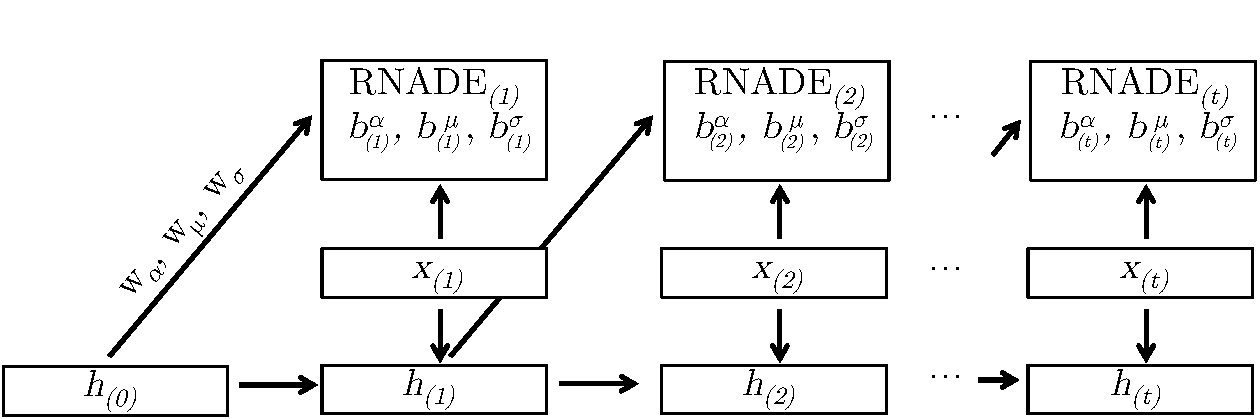
\includegraphics[scale=0.65]{RNN-RNADE.pdf}
    \caption{Graphical structure of the RNN-RNADE. The hidden state of the RNN at time $t$ predicts the parameters of the RNADE at $t+1$. }
    \label{fig:rnn-rnade}
\end{figure}


The RNN-RNADE is a sequence of conditional distributions for each time-step of a sequence $\mathbf{x}$. As shown in Figure \ref{fig:rnn-rnade}, the parameters of the conditional distributions at each time step, $t$, are a function of the hidden state of the RNN at the previous time-step, $t-1$. We first define the notation in order to simplify discussion of the training algorithm later in this section. 

From section \ref{RNADE}, the RNADE is parameterised by $ \theta \equiv \left\{ \mathbf{V}^{\alpha},\mathbf{V}^{\mu},\mathbf{V}^{\sigma},\mathbf{b}^{\alpha},\mathbf{b}^{\mu},\mathbf{b}^{\sigma} \right\}$. Let  $ \theta_t \equiv \left\{ \mathbf{V}^{\alpha}_{t},\mathbf{V}^{\mu}_{t},\mathbf{V}^{\sigma}_{t},\mathbf{b}^{\alpha}_{t},\mathbf{b}^{\mu}_{t},\mathbf{b}^{\sigma}_{t} \right\}$ denote the parameters of the conditional RNADE at time $t$. Although all the parameters of the RNADE at time $t$ can be a function of the hidden state at $t-1$, we consider the matrices $ \mathbf{V}^{\alpha},\mathbf{V}^{\mu},\mathbf{V}^{\sigma}$ to be fixed and only consider the biases $\mathbf{b}^{\alpha},\mathbf{b}^{\mu},\mathbf{b}^{\sigma}$ to be time-dependent through the RNN hidden state. This constraint significantly reduces the number of parameters that need to be estimated and makes the model and training computationally more efficient. 
Therefore, $ \theta_t \equiv \left\{ \mathbf{V}^{\alpha},\mathbf{V}^{\mu},\mathbf{V}^{\sigma},\mathbf{b}^{\alpha}_{t},\mathbf{b}^{\mu}_{t},\mathbf{b}^{\sigma}_{t} \right\}$. 

The time-dependent RNADE parameters are given by:
\begin{equation}
\label{one}
\rvec(\mathbf{b}^{\alpha}_{t}) = \rvec(\mathbf{b}^{\alpha}) + W_{\alpha}\mathbf{h}^{t-1}
\end{equation}
\begin{equation}
\label{two}
\rvec(\mathbf{b}^{\mu}_{t}) = \rvec(\mathbf{b}^{\mu}) + W_{\mu}\mathbf{h}^{t-1}
\end{equation}
\begin{equation}
\label{three}
\rvec(\mathbf{b}^{\sigma}_{t}) = \rvec(\mathbf{b}^{\sigma}) + W_{\sigma}\mathbf{h}^{t-1}
\end{equation}
where $\rvec(A) = [a_{1,1}, ..., a_{1,n}, a_{2,1}, ..., a_{2,n}, ..., a_{m,1}, ..., a_{m,n}]$ for some $m \times n$ matrix $A$, $W_{\alpha},W_{\mu},W_{\sigma} \in \mathbb{R}^{r \times D c}$ are the weights from the hidden state of the RNN to the mixing coefficients, means and standard deviations of the RNADE respectively, $r$ is the number of hidden units in the RNN, $D$ is the dimensionality of the input vectors and $c$ is the number of components of each GMM in the RNADE. 

%Therefore using equations \ref{one},\ref{two},\ref{three} we can obtain the time-dependent biases for the RNADE at each time step. 

\subsection{Learning in the RNN-RNADE}

The model can be trained by minimising the negative log-likelihood of training sequences using gradient descent. The cost function is given by:
\begin{align}
L(\theta) &= - \log P(\mathbf{x}) \nonumber\\ 
&= -\sum_{t=1}^{T} \log P(\mathbf{x}^t;\theta^t) \label{cost}
\end{align}

The gradients of the conditionals $P(\mathbf{x}^t;\theta^t)$ with respect to the parameters of the RNADE can be calculated, the details of which are outlined in \cite{Uria2013}. Once we obtain the gradients with respect to the time-dependent parameters, the entire network can be trained using BPTT. 

From Equation \ref{cost}, $\frac{\partial L}{\partial \mathbf{b}^{\alpha}_{t}} = \frac{\partial (-P(\mathbf{x}^t;\theta^t))}{\partial \mathbf{b}^{\alpha}_{t}}$ which can be obtained as shown in \cite{Uria2013}. The derivatives of the cost with respect to the other time-dependent parameters can be obtained in a similar manner. Once we obtain $ \frac{\partial L}{\partial \mathbf{b}^{\alpha}_{t}}, \frac{\partial L}{\partial \mathbf{b}^{\mu}_{t}}, \frac{\partial L}{\partial \mathbf{b}^{\sigma}_{t}}$, the gradients with respect to the other model parameters can be calculated as follows:

\begin{equation}
\frac{\partial L}{\partial W_{\alpha}} = \sum_{t=1}^T \frac{\partial L}{\partial \mathbf{b}^{\alpha}_{t}} {\mathbf{h}^{t-1}}^{T}
\end{equation}
\begin{equation}
\frac{\partial L}{\partial W_{\mu}} = \sum_{t=1}^T \frac{\partial L}{\partial \mathbf{b}^{\mu}_{t}} {\mathbf{h}^{t-1}}^{T}
\end{equation}
\begin{equation}
\frac{\partial L}{\partial W_{\sigma}} = \sum_{t=1}^T \frac{\partial L}{\partial \mathbf{b}^{\sigma}_{t}} {\mathbf{h}^{t-1}}^{T}
\end{equation}

Using equations \ref{rnn-hidden},\ref{one},\ref{two},\ref{three}:

\begin{equation}
\label{grad-hidden}
\frac{\partial L}{\partial \mathbf{h}^t} = W_{rec}\frac{\partial L}{\partial \mathbf{h}^{t+1}} \mathbf{h}^{t+1} (1 - \mathbf{h}^{t+1}) + W_{\alpha} \frac{\partial L}{\partial \mathbf{b}^{\alpha}_{t+1}} + W_{\mu} \frac{\partial L}{\partial \mathbf{b}^{\mu}_{t+1}} + W_{\sigma} \frac{\partial L}{\partial \mathbf{b}^{\sigma}_{t+1}}
\end{equation}

Using equation \ref{grad-hidden}, the gradients with respect to the remaining model parameters can be calculated easily. 

$$ \frac{\partial L}{\partial \mathbf{b}_{h}} =  \sum_{t=1}^{T} \frac{\partial L}{\partial \mathbf{h}^t} \mathbf{h}^t (1 - \mathbf{h}^t)$$
$$ \frac{\partial L}{\partial W_{rec}} = \sum_{t=1}^{T} \frac{\partial L}{\partial \mathbf{h}^t} \mathbf{h}^t (1 - \mathbf{h}^t) {\mathbf{h}^{t-1}}^T$$
$$ \frac{\partial L}{\partial W_{in}} = \sum_{t=1}^{T} \frac{\partial L}{\partial \mathbf{h}^t} \mathbf{h}^t (1 - \mathbf{h}^t) {\mathbf{x}^{t}}^T$$

As shown above, the gradients of the cost function with respect to the model parameters can be obtained with BPTT and used to train the joint model. In our implementation of the model, we used the automatic differentiation library Theano \cite{bergstra+al:2010-scipy} instead of calculating the gradients by hand. In the supplementary material, we provide further details about the exact form of the gradients. Unlike the RNN-RBM, the gradients of the RNN-RNADE model can be calculated exactly. Therefore model training can benefit from the use of a more powerful gradient based optimiser like the Hessian Free optimiser \cite{Martens2011}.

\section{Experiments}
\label{Experiments}
The RNN-RNADE is tested on three tasks, a simple stochastic trajectory of the simulated motion of a point in 2-D space, motion capture data ({\it mocap}) and videos of bouncing balls. On all three tasks we report the squared prediction error, allowing comparisons between our approach and the RTRBM and RNN-RBM in the latter two tasks. We report the mean of the sum of the squared prediction errors per frame over 100 test sequences. 10 vectors are sampled from the predicted conditional distributions at each time step, and the mean squared error is calculated between the samples and the ground truth and summed over each dimension in the frame. This is averaged over 100 test sequences of length 100 (in Section 5.1 and 5.2) or 128 (in Section 5.3). Code for the experiments is available in the supplementary material.  A grid search was carried out on the hyperparameters, including the number of hidden neurons in the RNADE, the number of recurrent hidden neurons, the number of components and the learning rate. A new sequence is presented to the model for each parameter update and the system is set up for a maximum of 100,000 parameter updates. Early stopping was employed, comparing the model's score on a validation set. Additionally, training was halted if the log likelihood became positive.

%In all experiments, the RNADE was fixed to use 1 component per input dimension.

\subsection{2-D stochastic trajectory}
This task is used as a demonstrative example of the system. At each time step a particle's 2-D coordinates are determined by the system of equations:


$$x(t) \sim \mathcal{N}(\sin(t)+1,0.1) $$
$$ y(t) \sim x(t)\mathcal{N}(\sin(t)+0.5,0.2)$$


where $t$ is the timestep. The model is trained on sequences of 100 consecutive time steps. The model comprised of 20 hidden units for both the RNN and the RNADE. The motivation behind performing this task was to devise a toy problem for quickly evaluating the effects of changes made to the model or the training algorithm. Although the task is relatively easy and could be solved by simpler sequential models, visually inspecting predictions helped verify the effectiveness of the learning algorithm and isolate certain issues with training that are discussed in detail later in this section. Videos showing the predictions made by the model are attached in the supplementary material. As can be observed, the samples of the predicted conditional distributions produced by the model follow the path of the trajectory.

\subsection{Motion capture data}
As in \cite{Sutskever2008} and \cite{Boulanger-Lewandowski2012} we use the human motion capture dataset\footnote{http://people.csail.mit.edu/ehsu/work/sig05stf/} ({\it mocap}) which represents preprocessed sequences of 3-D joint angles and the rotation and displacement of the coccyx of a moving human subject. The data consists 49 real-valued dimensions at each time-step and is therefore ideal for evaluating the performance of the proposed model. As mentioned earlier, we performed a grid search on some of the hyper-parameters. The model that performed the best comprised of $100$ hidden units for the RNADE and $200$ hidden units for the RNN. The best squared prediction error was $\mathbf{7.26}$, which is a significant improvement over the RTRBM ($20.1$) and the RNN-RBM ($16.2$) as reported in \cite{Boulanger-Lewandowski2012}. 

\subsection{Videos of bouncing balls}
The bouncing balls dataset\footnote{www.cs.utoronto.ca/~ilya/code/2008/RTRBM.tar} consists of synthetic videos of three balls bouncing in a box, as described in \cite{Sutskever2008}. We used videos of 15x15 pixels (225 dimensions) of 3 balls bouncing and sequences of 128 frames. Each pixel is a real value in the range $[0,1]$. The RNADE is not an ideal distribution estimator for this problem since the input space is bounded but the GMMs at the RNADE outputs model are unbounded. In our experiments the best model comprised of $300$ hidden units for the RNN and $200$ hidden units for the RNADE. The best squared prediction error we achieved was $1.93$ which is a small improvement over the RTRBM ($2.11$) but worse compared to the RNN-RBM ($0.96$). In order to get a better understanding of the problem we inspected the samples produced by the conditional distributions. We observed that in a large proportion of frames there were a few samples which were very noisy, i.e. their values were much greater than 1 or much less than 0. These samples contributed to higher squared prediction errors. Clipping the samples drawn from the RNADE at $0$ and $1$ did not have any significant effect on the squared prediction error. We generated sequences of bouncing balls from the model similar to \cite{Sutskever2008}, However, the noisy samples (even with clipping) when used as inputs degrade the future samples quickly and we did not obtain smooth sequences. Videos showing samples generated from the model at the next time-step are attached in the supplementary material.

\section{Discussion}
\label{Discussion}
From the previous section we observe that the RNN-RNADE outperforms other models on real valued sequential data from the \textit{mocap} dataset. When the input space is bounded, the RNN-RNADE performs similarly to the RTRBM but is outperformed by the RNN-RBM. In this section we provide details of the training procedure and investigate some of the factors that impact performance. 
\subsection{Gradient Descent}
 The training algorithm was set to perform 100,000 updates, where one sequence was used to compute the gradients for the update. In our experiments we found that the model reached lower validation errors when momentum was used during gradient descent. We used a constant momentum rate of $0.9$ in all our experiments. We found that using high learning rates would either cause the gradients to blow up quickly or force the parameters to converge to local minima within a small number of epochs. We used an initial learning rate of $0.001$ and linearly decreased the learning rate to zero over 100,000 updates. 

Exploding or vanishing gradients is a well documented problem while training RNNs and was one of the primary reasons that research on RNNs stalled. In our initial experiments on the \textit{mocap} dataset we found that the gradients would explode even with very small learning rates. The problem of exploding gradients is likely to be more acute for the RNN-RNADE because of the highly non-linear relationship between the parameters of the RNN and the RNADE and the negative log-likelihood cost function. We used gradient clipping \cite{bengio2012advances} which deals with this problem using a simple heuristic. If the norm of the gradient $g$, for some update is above a threshold, then the gradient is rescaled to $(\frac{\tau}{\left\lVert g \right\rVert})g$, where $\tau$ is the threshold. In our experiments we set the threshold to 50, which was the average of the norm of the gradients of 1,000 randomly generated sequences. 

\subsection{Overfitting}
Although the training algorithm was set up to perform a large number of updates, on all three problems we noticed that the negative log-likelihood cost approaches zero very quickly. For example on the \textit{mocap} dataset, the cost approaches zero after 2,000 updates. Once the cost becomes negative, it can continue to reach arbitrarily low values without having much effect on the validation error. This demonstrates that the RNN-RNADE is prone to overfitting to the training data. The RNN-RNADE is more susceptible to this phenomenon than the RNADE or mixture density networks because the RNN is trying to accurately predict the mean at each time-step. As training progresses, the predictions from the RNN become more accurate and after a point the means are approximately equal to the data points causing the log-likelihood to become positive. It is not obvious how this problem can be dealt with since the means are functions of the hidden state of the RNN and the RNN gets better at predicting the means as training continues. This is a common issue when mixture density networks are trained via maximum likelihood estimation \cite{bishop2006pattern}. In an attempt to prevent the log-likelihood from becoming positive, we imposed an L2 penalty on the weight matrix from the RNN to the RNADE biases. With the tested penalties (between 0.1 - 10.0), this did not have any effect on the problem of overfitting. Having observed this, we used the training cost as a stopping criterion and stopped training when the log-likelihood becomes positive. However, even with this issue, the model learns very quickly (within 2,000 updates on the \textit{mocap} dataset) and still outperforms the RNN-RBM with a relative improvement of $55\%$. 

\subsection{Architecture}

As mentioned earlier, we only allow the bias parameters of the RNADE ($\mathbf{b}^{\alpha},\mathbf{b}^{\mu},\mathbf{b}^{\sigma}$) to be time-dependent. It is not clear a priori which combination of time dependent biases yields the optimal model for a given problem. In our experiments with the \textit{mocap} and bouncing balls datasets, we trained models with all possible combinations of time-dependent biases, with the obvious exception of the case where none of the biases are time-dependent. We observed that a time dependent $\mathbf{b}^{\mu}$ was crucial for the model to capture temporal dependencies. Whenever $\mathbf{b}^{\mu}$ was omitted from the set of time-dependent parameters, the model failed to learn. We found that time-dependent $\mathbf{b}^{\mu},\mathbf{b}^{\sigma}$ yielded the best models. Including $\mathbf{b}^{\alpha}$ in the set of time dependent parameters did not lead to better training, in fact a time dependent $\mathbf{b}^{\alpha}$ exacerbates the issue of overfitting during training. 

Another parameter that was crucial in determining test performance was the number of components in the GMMs at the RNADE output. GMMs when trained with a large number of components are known to cause overfitting \cite{bishop2006pattern}. We found that if we set the number of components to be greater than 2, then the model overfits very quickly during training and these models could not generalise to test data. Best results were obtained when the number of components was limited to $2$ components, with not much difference in performance between GMMs with $1$ or $2$ components.  

\section{Conclusions and Future Work}

In this paper we introduced the RNN-RNADE, a powerful probabilistic model for real-valued high dimensional sequences. We evaluated its performance and report a significant improvement in performance over previously proposed models from the same family on the \textit{mocap} dataset. The model can be trained with gradient descent and obtaining probabilities is tractable, unlike with other models. However, there are issues with the model that need to be investigated further. The model could potentially work much better if overfitting is avoided. More work is required to identify effective means of regularisation. There is also potential for improving training by using more powerful gradient based optimisers such as Hessian Free. 
\label{conclusion}

\section{Acknowledgements}

Removed for anonymity. 

\bibliography{bibliography}
\bibliographystyle{plain}
\end{document}
